%%%%%%%%%%%%%%%%%%%% author.tex %%%%%%%%%%%%%%%%%%%%%%%%%%%%%%%%%%%
%
% sample root file for your "contribution" to a proceedings volume
%
% Use this file as a template for your own input.
%
%%%%%%%%%%%%%%%% Springer %%%%%%%%%%%%%%%%%%%%%%%%%%%%%%%%%%


\documentclass{svproc}
\usepackage{marvosym}
%
% RECOMMENDED %%%%%%%%%%%%%%%%%%%%%%%%%%%%%%%%%%%%%%%%%%%%%%%%%%%
%
\usepackage{graphicx}
\usepackage{float}
\usepackage[boxed,vlined,ruled]{algorithm2e}

% to typeset URLs, URIs, and DOIs
\usepackage{url}
\usepackage{hyperref}
\def\UrlFont{\rmfamily}
\providecommand{\doi}[1]{doi:\discretionary{}{}{}#1}

\def\orcidID#1{\unskip$^{[#1]}$}
\def\letter{$^{\textrm{(\Letter)}}$}

%%%%%% DEBUG section %%%%%%
\newcommand*{\DEBUG}{}

\ifdefined\DEBUG
\usepackage[T2A]{fontenc}
\usepackage[utf8]{inputenc}
%\usepackage[russian]{babel}
\usepackage[usenames]{color}
%\usepackage{colortbl}
\newcommand{\FIXME}[1]{ % описание
	\colorbox{yellow}{#1}
}
\else
\newcommand{\FIXME}[1]{ % описание
}
\fi


\begin{document}
\mainmatter              % start of a contribution
%
\title{Topological approach to finding blackholes in directed networks}
%
\titlerunning{Topological black holes mining}  % abbreviated title (for running head)
%                                     also used for the TOC unless
%                                     \toctitle is used
%
\author{Denis Ivanov\inst{1} \and Alexander Semenov\inst{2}}
%
\authorrunning{Ivanov, Semenov} % abbreviated author list (for running head)
%
%%%% list of authors for the TOC (use if author list has to be modified)
\tocauthor{Denis Ivanov and Alexander Semenov}
%
\institute{Lomonosov Moscow State University, Moscow, Russian Federation \\
\email{mr.salixnew@gmail.com}
\and
JSC NICEVT, Moscow, Russian Federation\\
\email{semenov@nicevt.ru}
}

\maketitle              % typeset the title of the contribution

\begin{abstract}
In this paper we consider the task of finding so called Blackhole pattern in directed unweighed graphs.
Firstly, we analyse already existing algorithms and approaches. Secondly, we describe how structure of a graph
affects their efficiency. Then we introduce our approach to graph preprocessing. Finally, we describe topological sort based heuristic
and provide results of experimental comparison between our approach and previously developed algorithm.
% We would like to encourage you to list your keywords within
% the abstract section using the \keywords{...} command.
\keywords{Directed networks $\cdot$ Subgraph mining}
\end{abstract}

\section{Blackhole Search in Directed Graph}
The task of pattern mining in directed graphs finds its aplications in different areas. In 2010 Li et al.\cite{li2010mining} state
that governments are interested in detecting cases of financial fraud. They formulate the task for finding cases of illegal collaboration, and introduce dual patterns:
blackhole and volcano. Those appear when a group of traders perform operations only between each other in order to manipulate market.
Continuing study of different financial fraud casese, in 2017 Semenov et al. \cite{semenov2017survey} provided a survey of common approaches to anti - money laundering by graph mining.
There are other applications. For example, the online detection of black holes/volcanos can timely 
reflect anomalous events, such as disasters, catastrophic accidents, and therefore help keep public safety \cite{hong2015detecting}.

\subsection{Problem Statement and Preliminaries}
In this section we provide some basic notations and definitions, which will be used in this paper. In this paper we consider simplified problem formulation, applied to directed unweighted graph.

First, consider a directed graph $G = G(V,E)$, where $V$ is a set of all nodes and $E$ is a set if all edges of the graph. 
\FIXME{Мне кажется, это лишнее предложение, так не пишут в статьях:} Assume that we deal with the general case of graph, without any special restrictions, unless the opposite is stated. 

\begin{definition}
Subset of nodes $B \in V$ is called a blackhole if  the following two conditions are satisfied: 
1) Subgraph $G'(B, E')$ induced by $B$ is weakly connected, 
%$|B| \geq 2$,
and
2) there is no such pair of nodes $(u,v)$ that $u \in B$, $v \in V \backslash B$ and $(u,v) \in E$.
\end{definition}

The goal is to find in unweighted directed graph as many blackholes as possible in restricted time.

To support further discussion, we provide several more definitions.

\FIXME{Удалил возможные кратные ребра в определении 2, это важно?}
\begin{definition}
For a given directed graph $G(V,E)$ we say that sequence $v_0v_1v_2...v_{k}$ of $v_i \in V, 0 \leq i \leq k$ forms a directed path from $v_0$ to $v_k$, if there are edges $(v_{i-1}, v_i) \in E, 1 \leq i \leq k$ and $v_i \neq v_j$ for all $0 \leq i, j \leq k, i \neq j$. The length of this directed path is $k$.
\end{definition}

\begin{definition}
For a given directed graph $G(V,E)$ we say that $v \in V$ is reachable from $u \in V$ if there is a directed path that starts from $u$ and ends at $v$.
\end{definition}

\begin{definition}
For a given directed graph $G(V,E)$ if $v \in V$ is reachable from $u \in V$, then we say $u$ is a predecessor of $v$ and $v$ is a successor if $u$.
If there is an edge from $u$ to $v$, then $u$ is a direct predecessor of $v$, and $v$ is a direct successor if $u$.
\end{definition}

\begin{definition}
Set of nodes in a directed graph $G$ is called a Strongly Connected Component (SCC) if every node of $G$ is reachable from every other node of $G$.
\end{definition}

\begin{definition}
For a given directed graph $G(V,E)$. The closure of $v \in V$ is $Closure(v) = \{u\ |\ there\ is\ a\ directed\ path\ from\ v\ to\ u\} \cup \{v\}$.
In other words, a closure of node $v$ is a set of all nodes reachable from $v$, including $v$.
\end{definition}

The following lemmas are proved in \cite{li2010detecting}.

\begin{lemma}
If a node $v \in B$, where $B \subseteq V$ is a blackhole, then all the successors of $v$ are in $B$.
\end{lemma}

\begin{lemma}
If a node $v \in B$, where $B \subseteq V$ is a blackhole, then the closure of $v$ is a subset of $B$.
\end{lemma}

\begin{lemma}
Closure of $v$ forms a blackhole.
\end{lemma}

We will need the following statement to discuss issues of known approaches.
\begin{lemma}
For a given graph $G(V,E)$, SCC $S \subseteq V,\ blackhole\ B \subseteq V$ if $\ \exists v \in S: v \in B$,  then $\forall s \in S$ will be true $s \in B$.
In other words, if any node in SCC belongs to a blackhole, then all the nodes of this SCC belong to the same blackhole.
\end{lemma}
\begin{proof}
    In SCC any node is reachable from any other node. This means, that any node $v$ in SCC contains the whole SCC in its closure. By Lemma 3 the whole SCC belongs to the same blackhole as $v$. 
\end{proof}

\subsection{Related Work}

% Previously 
%Authors from the University of New Jersey gave \cite{li2010detecting} general and simplified problem formulation for blackhole search
in directed graph.

The main contributor to the blackhole detecting problem is the authors from the University of New Jersey. They both formulated the task and provided an algorithm for blackhole detection in case of unweighted directed graph \cite{li2010detecting}. 
Two years later they published an algorithm for approximate blackhole search in general case (weighted graph) \cite{li2012mining,li2014mining}. 
Hong et al \cite{hong2015detecting} had
an unusual application for blackhole mining in the city environment. They introduced an original algorithm.  

\subsection{Known issues}
In this section we shortly discuss applicability of iBlackhole algorithm.
iBlackhole \ref{alg:iblackhole} algorithm is designed for searching blackholes of fixed size. It has a great resource of parallelism, which is demonstrated
by tests. However, survey by Li et al, doesn't cover case of large scale graphs, as they only run their algorithm on 1500 node networks, which seem quite
a small size.
Also, it is worth mentioning that there are graphs, which has a small amount of blackholes in relation to number of nodes. They consist
of several large SCCs and relatively small amount of independent leaves (or roots). Here arise some questions considering applicability of
iBlackhole algorithm:
\begin{itemize}
\item How do we know if there are blackholes of certain size? We have to check all the possible sizes, which can take too long even in parallel.
\item If we check blackhole sizes consecutively, what is the expected time of the first blackhole found?
\item How do we reduce search field for the BruteForce stage and avoid repeatedly checking the same combinations for different sizes?
\end{itemize}

Let's consider the following example:

Graph consisting of $(10^6)$ nodes, all of them form a single SCC. It means that there is only one blackhole - the whole graph.
Unless we do not know anything about the graph structrure and do not have large enough cluster, we have one to a million chance
to efficiently choose target size of blackhole. In general case, we have to check $10^6$ possible sizes.

Another example is common SmallWorld \cite{watts1999networks} graph. It has most of its nodes in one large SCC, couple of leaves and couple of roots.
With iBlackhole algorithm and consequtive approach we will quickly discover all the small blackholes and then for a long time will try to discover
blackholes inside an SCC.

\begin{figure}[H]
	\begin{center}
		\begin{algorithm}[H]
			\SetAlgoLined
			\SetKwInOut{Input}{Input}
			\SetKwInOut{Output}{Output}
			\Input{$G$ -- directed graph \\
                                $V$ -- set of all nodes \\
                                $E$ -- set of all edges \\
                                $n$ -- max number of nodes each blackhole can contain}
			\Output{$Blackhole$ -- 1 to n-node blackhole set of G}

                        $Blackhole = \emptyset$ \\
                        \For{$i = 1\ to\ n$} {
                            $P_i = \{v | d_{out}(v) < i\}$ \\
                            \ForEach{$v \in P_i$} {
                                \If{$v \notin C_{i-1}$} {
                                    \If{$at\ least\ one\ of\ v's\ directed\ successors\ are\ not\ in\ P_i$} {
                                        $remove\ v\ from\ P_i$\\
                                        $remove\ all\ v's\ predecessors\ from\ P_i$\\
                                    }
                                }
                            }
                        }
                        $C_i = P_i$\\
                        \ForEach{$v \in C_i$} {
                            \If{$|Closure(v)| == i$} {
                                $Blackhole = Blackhole \cup Closure(v)$
                            }
                            \If{$|Closure(v)| >= i$} {
                                $remove\ v\ from\ C_i$ \\
                                $remove\ all\ v's\ predecessors\ from\ C_i$ \\
                            }
                        }
                        $F_i = C_i$\\
                        \ForEach{$B \in F_i(i)$} {
                            \If{$G(B)\ is\ weakly\ connected$} {
                                \If{$d_{out}(B) == 0$} {
                                    $Blackhole = Blackhole \cup B$ \\
                                }
                            }
                        }
                        \Return $Blackhole$
			\label{alg:iblackhole}
			\caption{iBlackHole}
		\end{algorithm}
	\end{center}
\end{figure}

\section{Algorithm design}
We propose to look at the blackhole search problem from the following: it would be divided into two independent tasks. 
The first one is graph preprocessing. Here we aim to simplify graph structure as far as it is possible with respect to a restricted time span. 
Decreased graph scale would definitely speed up the the calculation, as it can fall into a brute-force search in most cases.
The second is the blackhole search itself. This step is done after preprocessing and the goal here is to find as many blackholes as possible in a restricted time.

%
\subsection{Graph preprocessing}
\FIXME{не забыть вставить ссылки SmallWorld \cite{watts1999networks}}

As it was described in the Known issues section, large SCCs waste lots of computational time without adding any new blackholes. 
For certain graph types (RMAT, SmallWorld\cite{watts1999networks}) it can be crucial, because one SCC can contain up to 100\% of all graph's nodes. 
In such a case, it would be nice to consider large SCC as a single node, aggregating all incoming and outcoming peripheral edges
of original SCC.
On the preprocessing stage of the algorithm we reduce every SCC to a single node. The algorithm is not new and known as a graph condensation.
More formally:

\begin{definition}
If every SCC of directed graph is contracted to a single node, the resulting graph is directed acyclic graph, which is call the condensation of G.
\end{definition}

In this article we use the following algorithm for finding graph condensation. \ref{alg:condensation}
It was independently proposed by Kosaraju and Sharir back in 1979. \FIXME{Ссылку на эту статью}

First, we find topological sort of the initial graph..

\begin{definition}
Topological sort or topological ordering of a directed graph is a linear ordering of 
its vertices such that for every directed edge $(u,v)$ from node $u$ to node $v$,
$v$ comes before $u$ in the ordering.
\end{definition}


\begin{definition}

\end{definition}

When we finally have an array, containing graph nodes in the topologically sorted order, we do the following:

Define global array of used nodes. Initially, all nodes are unused.
Then for every node from bottom to top:
\begin{enumerate}
    \item Acquire closure of unused nodes reachable from current node; 
    \item Mark every node in the closure as used;
    \item All the acquired nodes belong to the same SCC.
\end{enumerate}

The fact given in the last step can be shortly explained in the following way:
topological sort guarantees that any node has index larger than indeces of her children.
That is why, given that we process nodes from bottom to top, by the moment we process the node, all it's children are already marked used and no longer available for search.
As all the ways down are prohibited and there's no way up, we will acquire an SCC.

\begin{figure}[H]
	\begin{center}
		\begin{algorithm}[H]
			\SetAlgoLined
			\SetKwInOut{Input}{Input}
			\SetKwInOut{Output}{Output}
			\Input{$G(V,E)$ -- directed graph}
			\Output{$G'(V',E')$ -- directed acyclic graph }
                        $tsOrder = TopSort(G)$ \\
                        $scc = [-1\ for\ i = 1\ to\ |V|] $ \\ 
                        $component = 0$ \\
                        \ForEach{$v \in tsOrder$} {
                            \If{$scc[v] == -1$} {
                                $C_v = Closure(v)$ \\
                                \ForEach{$u \in C_v$} {
                                    $scc[u] = component$ \\
                                }
                                $component = component + 1$ \\
                            }
                        }

                        $E' = \emptyset$ \\
                        $V' = \emptyset$ \\
                        \ForEach{$(u,v) \in V \times V$} {
                            \If{$scc[u] \neq scc[v]$} {
                               $V' = V' \cup \{scc[u], scc[v]\}$ \\ 
                               $E' = E' \cup (scc[u], scc[v])$ \\ 
                            }
                        }
                        \Return $G'$
			\label{alg:condensation}
			\caption{Graph condensation. Kosarayu, Sharir}
		\end{algorithm}
	\end{center}
\end{figure}

As a result of the algorithm, described above, we have each node associated with certain SCC.
SCCs itself form a graph with number of nodes less than or equal to one of the initial graph.
Finally, we need to remove edges duplicates and the graph condesation is built.

%

%
\subsection{Blackholes Search}
When the graph is prepared, we can move on to searching blackholes. The problem is combinatorial in its nature, therefore, we aim to
decrease the number of potential blackholes.
To understand the issue, we first describe a brute-force approach. 

\begin{definition}{Root of blackhole.\\}
Root of blackhole(subgraph) is a node, which has no incoming edges from other nodes in blackhole.
\end{definition}

\begin{definition}{Blackhole basis. \\}
Set of all roots of blackhole is called blackhole basis
\end{definition}

\begin{definition}{Simple blackhole. \\}
A blackhole is called simple if its basis consists of a single node, i.e. it has single root.
\end{definition}

\begin{definition}{Complex blackhole. \\}
A blackhole is called complex if its basis consists of more than one node.
\end{definition}

%TODO: осознать
In the BruteForce algorithm we iterate over all possible unordered sets of nodes. 
Then for every node we acquire its closure. Union of all such closures is a potential blackhole.
If the candidate blackhole is a weakly connected subgraph, then it is a blackhole.

With the BruteForce algorithm it is possible to find the same blackhole several times.
We aim to avoid at least some of the duplicates and introduce heuristic for it.

According to the definitions above if some node is not a root of a blackhole, it can be omitted, as set of roots uniquely identify a blackhole.
Every non-root node in a blackhole is reachable from one of the roots. Therefore, if we know reachability matrix for a given graph, we can skip bloated non-basis combinations of nodes.

Of course, we could straightforward build the reachability matrix. But, it takes $O(V^3)$ time. Even though we decreased graph size
in preprocessing step, it still can result in lots of computation. It's worth mentioning that ultimate goal is to find at least some blackholes as soon as possible. 
Difficult precalculation will affect the time of first blackhole discovery. That is why, we will only try to partially skip duplicates and the rest will
be filtered later in lazy manner.

Let's consider a closure of a single blackhole root. Let this closure to be acquired by depth-first search, which basically means, that
we can iterate over these nodes in topologically sorted order. Also, while traversing this graph, we can calculate size of closure for each node
in the given roots closure. Finally, if some node is in the $i$-th position of the topological sort and its closure size is $i$, then we can 
conclude, that every node with index less than $i$ in the topological sort will be reachable from $topsortOrder[i]$. We will call such nodes special.

If there are two special nodes under the same root, union of their closures will be equal to the closure of topologically higher node.
Hence, union of closures for any subset of special nodes under the same root will result into closure of the highest special node.

Let's consider two nodes in the closure of global root. One of them is non-special, the other one is special. In order for these two nodes to be basis
special one should be topologically lower than non-special. Otherwise it would be one node basis.
To sum up: if given a set of nodes, we shall remove nodes topologically lower than highest ones special nodes in every global root closure.

Imagine, we are given a graph and a set of nodes. What is the algorithm to decide whether these nodes form the basis of a blackhole? We shall decide if there's at least
one non-basic node. It's done by \ref{alg:isbasis}
\begin{enumerate}
    \item First, we need to know what special nodes there are. This step can be precalculated. 
    To find out, we will take every global root of condensated graph and find topoological sort of its closure.
    Those vertices, which suffice the rule above, we will mark as "special". 
    \item Now, we shall calculate how many special nodes for every root there is in the given set. If there is more than one special node for root - the set is to be called non-basis and
    omitted.
    \FIXME{partially implemented: по факту тут алгоритм применяется только к первому корню. Это было проще реализовать. }
    \item Also we shall check if there are any non-special nodes lower than the special ones in related root topsort order, and if those found - omit the node set.
    \item When we are out of heuristics, we check if any of the candidate nodes are reachable from one another. If so, omit this set. 
    \FIXME{partially implemented: здесь условие выглядит несколько иначе: в упорядоченном наборе кандидатов специальная вершина может быть только первой. Впрочем, возможно, что тут баг. }
    \item Otherwise, we have a valid basis of a blackhole.
    To acquire blackhole we should, according to definition of basis, unite all the closures of basic nodes.
    Finally, we check for weak connectivity and if it is present - print blackhole.
\end{enumerate}

\begin{remark}
Of course, we still have to spend some computation time in order to decide, whether
the candidate is worth checking or not, and we understand, that sometimes it can make process even more slower than before, but experimental results demostrate its efficiency.
Our goal is to avoid this costly procedure of acquiring blackhole if possible.
\end{remark}

\begin{figure}[H]
	\begin{center}
		\begin{algorithm}[H]
			\SetAlgoLined
			\SetKwInOut{Input}{Input}
			\SetKwInOut{Output}{Output}
			\Input{$G(V,E)$ -- directed acyclic graph (Graph condensation) \\
                                $Cand(G)$ -- set of nodes; candidate to be basis}
			\Output{$True/False$}
                        // (1) precalc special nodes for every root \\
                        \ForEach{$r \in Roots(G)$} {
                            $Special_r = \emptyset$ \\
                            $tsOrder_r = TopSort(r)$ \\
                            \For{$i = 0; i<|tsOrder_r|; i=i + 1$} {
                                $v = tsOrder_r[i]$ \\
                                $C_v = Closure(v)$ \\
                                \If{$|C_v| == i$} {
                                    $Special_r = Special_r \cup v$ \\
                                }
                            }
                        }
			// (2) check for excluding specials \\
			\ForEach{$v \in Cand(G)$} {
                            \ForEach{$r \in Roots(G)$} {
                                \If{$v \in Special_r$} {
                                    $Spec_r = Spec_r \cup v$ \\
                                    \If{$|Spec_r| > 1$} {
                                        \Return $False$ \\
                                    }
                                }
                            }
			}
                        // (3) Check for candidates reachable from one another \\
                        \ForEach{$(v, u) \in Cand(G) \times Cand(G)$} {
                            \If{v is reachable from u} {
                                \Return $False$ \\
                            }
                        }
                        \Return $True$
			\label{alg:isbasis}
			\caption{BasisOrNot}
		\end{algorithm}
	\end{center}
\end{figure}

\begin{figure}[H]
	\begin{center}
		\begin{algorithm}[H]
			\SetAlgoLined
			\SetKwInOut{Input}{Input}
			\SetKwInOut{Output}{Output}
			\Input{$G(V,E)$ -- directed graph}
			\Output{$Blackhole$ -- set of blackholes of different sizes}
                        
                        $Blackhole = \emptyset$\\
                        $Build\ graph\ condensation\ Cond(V',E')$\\
                        \For{$i = 1\ to\ |V'|$} {
                            \ForEach{$B_i \in V'(i)$} {
                                \If{$BasisOrNot(Cond(V',E'),B_i)$} {
                                    \If{$B_i$\ is\ weakly\ connected} {
                                        $BlackHole = Blackhole \cup B_i$ \\
                                    }
                                }
                            }
                        }
                        \Return $Blackhole$
			\label{alg:topsort}
			\caption{TopSort}
		\end{algorithm}
	\end{center}
\end{figure}

%
\section{Experimental Results}
To demonstrate efficiency of our approach, we conducted a series of experiments. We ran the both algorithms (New Jersey \ref{alg:iblackhole} and TopSort ) on a 
set of graphs. 

iBlackhole algorithm was implemented in accordance with the pseudocode in the original article. Divide and Conquer heuristic were not used for it.
Our algorithm first applies condensation-based preprocessing and then uses BruteForce with partial reachability heuristic implemented via topsort.
Both algorithms filter duplicates 

For these experiments we chose Uniform Random (UR) \cite{random-uniform}, RMAT \cite{chakrabarti2004r},  and SSCA2 \cite{bader2005design} graph types. Those were generated for scales from 4 to 22
with step 2. Size $i$ means that graph has $2^i$ nodes and $32*V$ edges. Actual count of edges to process can differ from these ideal values, as duplicate edges and self-loops are omitted when readinggraph from file. Configuration of the considered graphs is presented in Table \ref{tabular:graphs}.

\begin{table}[]
\caption{Configuration of experimental graphs}
\label{tabular:graphs}
\begin{center}
\begin{tabular}{c|c|c}
Graph Type & Nodes Count & Edges Count \\
\hline
RMAT.04 & 16 & 177 \\
RMAT.06 & 64 & 1270 \\
RMAT.08 & 256 & 6663 \\
RMAT.10 & 1024 & 30186 \\
RMAT.12 & 4096 & 126988 \\
RMAT.14 & 16384 & 517554 \\
RMAT.16 & 65536 & 2087072 \\
RMAT.18 & 262144 & 7892410 \\
RMAT.20 & 1048576 & 32993233 \\
RMAT.22 & 4194304 & 67099679 \\
SSCA2.04 & 16 & 120 \\
SSCA2.06 & 64 & 722 \\
SSCA2.08 & 256 & 2668 \\
SSCA2.10 & 1024 & 10529 \\
SSCA2.12 & 4096 & 43603 \\
SSCA2.14 & 16384 & 173477 \\
SSCA2.16 & 65536 & 677649 \\
SSCA2.18 & 262144 & 2724762 \\
SSCA2.20 & 1048576 & 10902287 \\
SSCA2.22 & 4194304 & 43580024 \\
UR.04 & 16 & 207 \\
UR.06 & 64 & 1614 \\
UR.08 & 256 & 7652 \\
UR.10 & 1024 & 32201 \\
UR.12 & 4096 & 130486 \\
UR.14 & 16384 & 523740 \\
UR.16 & 65536 & 2096570 \\
UR.18 & 262144 & 8388074 \\
UR.20 & 1048576 & 33553908 \\
UR.22 & 4194304 & 134217174
\end{tabular}
\end{center}
\end{table}

We have been conducting our experiments on a Linux machine with the following specifications:
\begin{itemize}
    \item CPU: Intel Core i7-8550U CPU @ 4GHz
    \item RAM: 15802 MiB
    \item OS: Ubuntu 16.04 xenial
    \item Kernel: x86\_64 Linux 4.15.0-46-generic
    \item Shell: bash 4.3.48
\end{itemize}

All runs were performed in a single-thread mode. We allowed up to 20 minutes of working time for every run. In order to save time,
algorithms did not print out found blackholes, but printed counter on every found and not filtered (by any reason) blackhole.

Please, mention, that "blackhole found" means that we have a set of vertex numbers in memory ready to be printed out and it's already validated.

As it is shown in the Tables \ref{tabular:tableresults}, \ref{tabular:tableresults2}, our TopSort approach to blackhole search shows better perfoermance on small RMAT graphs.
And it stays in advantage up to RMAT-22. Apparently, condensation preprocessing takes more time on larger graphs and increases time spent before finding
the first blackhole. Nevertheless our algorithm shows significantly better performance in those cases when preprocessing saves more time. Also, we suppose
that total working time on large graphs for our algorithm will be less, and this is the point for future survey.

\FIXME{Это, вообще говоря, странно}
SSCA2 graphs in our survey can be characterized with absolute absence of SCCs consisting of more than one node. Preprocessing here doesn't give any
certain advantage, but only takes time. As we can see, on smaller graphs our approach beats iBlackhole algorithm, but slows down on larger graphs.
We guess that the reason is less efficient order of search for our algorithm. One used in iBlackHole will faster print smaller balckholes, and later will try
to find larger ones, meanwhile our approach will check blackholes of all sizes.

Finally, we should point out, that our preprocessing dramatically speeds up blackhole search on the graphs, where no blackholes present at all. Brute force is
avoided completely in this case, making calculation time impressively small in comparison to iBlackhole algorithm.

\begin{table}[]
\caption{Experimental results}
\label{tabular:tableresults}
\begin{center}
\begin{tabular}{c|c|c|c|c|c|c|c|c}
Graph & Type & Algorithm & Blackholes & Time(s) & Algorithm & Blackholes & Time(s) \\
\hline
RMAT & 04 & NewJersey & 1 & 0.000265422 & TopSort & 1 & 0.000115912 \\
RMAT & 06 & NewJersey & 1 & 0.0121347 & TopSort & 1 & 0.00034812 \\
RMAT & 08 & NewJersey & 1 & 1.66685 & TopSort & 1 & 0.00146486 \\
RMAT & 10 & NewJersey & 6 & 1200 & TopSort & 10 & 0.00684045 \\
RMAT & 12 & NewJersey & 29 & 1200 & TopSort & 971738 & 1200 \\
RMAT & 14 & NewJersey & 187 & 1200 & TopSort & 735128 & 1200 \\
RMAT & 16 & NewJersey & 1192 & 1200 & TopSort & 373705 & 1200 \\
RMAT & 18 & NewJersey & 5176 & 1200 & TopSort & 10286 & 1200 \\
RMAT & 20 & NewJersey & 617 & 1200 & TopSort & 48867 & 1200 \\
RMAT & 22 & NewJersey & 98 & 1200 & TopSort & 0 & 1200 \\
SSCA2 & 04 & NewJersey & 16 & 0.154763 & TopSort & 16 & 0.000189925 \\
SSCA2 & 06 & NewJersey & 11 & 1200 & TopSort & 70 & 0.00121528 \\
SSCA2 & 08 & NewJersey & 42 & 1200 & TopSort & 263314 & 1200 \\
SSCA2 & 10 & NewJersey & 85 & 1200 & TopSort & 114411 & 1200 \\
SSCA2 & 12 & NewJersey & 343 & 1200 & TopSort & 5870 & 1200 \\
\end{tabular}
\end{center}
\end{table}

\begin{table}[]
\caption{Experimental results. Part 2}
\label{tabular:tableresults2}
\begin{center}
\begin{tabular}{c|c|c|c|c|c|c|c|c}
Graph & Type & Algorithm & Blackholes & Time(s) & Algorithm & Blackholes & Time(s) \\
SSCA2 & 14 & NewJersey & 1433 & 1200 & TopSort & 323671 & 1200 \\
SSCA2 & 16 & NewJersey & 5829 & 1200 & TopSort & 893376 & 1200 \\
SSCA2 & 18 & NewJersey & 23179 & 1200 & TopSort & 224567 & 1200 \\
SSCA2 & 20 & NewJersey & 92347 & 1200 & TopSort & 24199 & 1200 \\
SSCA2 & 22 & NewJersey & 370770 & 1200 & TopSort & 0 & 1200 \\
UR & 04 & NewJersey & 1 & 0.000223768 & TopSort & 1 & 0.000115029 \\
UR & 06 & NewJersey & 1 & 0.0170713 & TopSort & 1 & 0.000331235 \\
UR & 08 & NewJersey & 1 & 2.30256 & TopSort & 1 & 0.00147483 \\
UR & 10 & NewJersey & 1 & 240.822 & TopSort & 1 & 0.00670724 \\
UR & 12 & NewJersey & 0 & 1200 & TopSort & 1 & 0.034011 \\
UR & 14 & NewJersey & 0 & 1200 & TopSort & 1 & 0.47257 \\
UR & 16 & NewJersey & 0 & 1200 & TopSort & 1 & 3.05003 \\
UR & 18 & NewJersey & 0 & 1200 & TopSort & 1 & 14.5788 \\
UR & 20 & NewJersey & 0 & 1200 & TopSort & 1 & 67.7176 \\
UR & 22 & NewJersey & 0 & 1200 & TopSort & 1 & 373.244
\end{tabular}
\end{center}
\end{table}
\pagebreak

\section{Conclusion}

\textit{Comment for the reviewer}. In the final paper revision we add parallel implementation of the TopSort algorithm and present much detailed evaluation on the larger graphs. 

In this paper we formulated and addressed some issues in application of already known iBlackhole algorithm. We introduced and tested two different ideas of optimization, combined into
our TopSort algorithm. Those are: graph condensation preprocessing and topsort bruteforce optimization. We tested out approach on three different types of graphs and number of scales.
In case of large SCCs we demostrate definite advantage over iBlackhole algorithm. Then, we can relatively fast detect total absence of blackholes, but sometimes quite costly preprocessing
deminishes any boost of productivity and out performance degrades.

%
% ---- Bibliography ----
%
\bibliographystyle{spmpsci}
\bibliography{biblio}

\begin{figure}[p]
    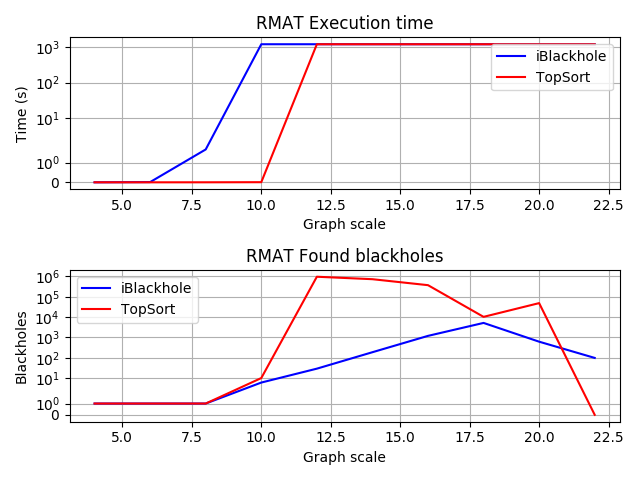
\includegraphics[width=\linewidth]{rmat.png}
    \caption{RMAT}
    \label{fig:rmat}
\end{figure}
\begin{figure}[p]
    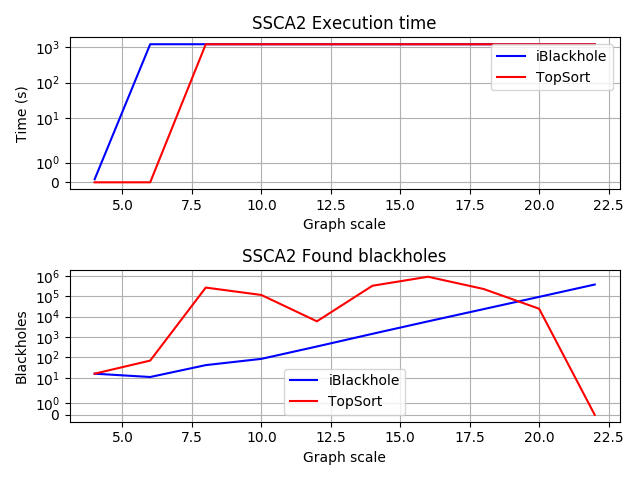
\includegraphics[width=\linewidth]{ssca2.png}
    \caption{SSCA2}
    \label{fig:ssca2}
\end{figure}
\begin{figure}[p]
    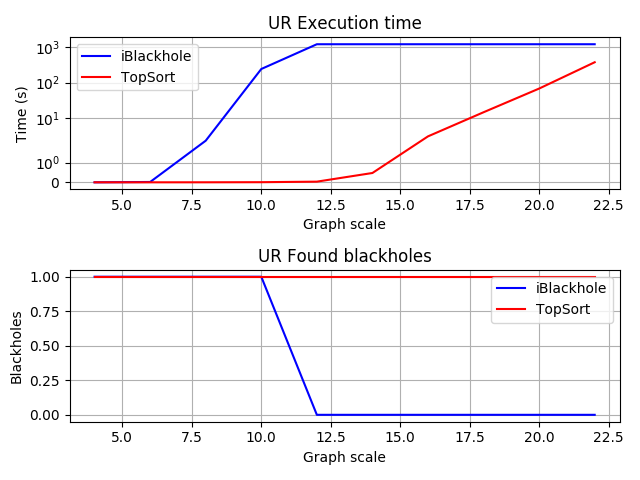
\includegraphics[width=\linewidth]{ur.png}
    \caption{UR}
    \label{fig:ur}
\end{figure}

\end{document}
